\chapter{Conexidad fuerte}

\index{strongly connected graph}

En un grafo dirigido,
las aristas se pueden recorrer en una sola dirección,
por lo que aunque el grafo sea conexo,
esto no garantiza que exista
un camino de un nodo a otro nodo.
Por esta razón, tiene sentido definir un nuevo concepto
que requiere más que conexidad.

Un grafo es \key{fuertemente conexo}
si hay un camino desde cualquier nodo a todos
los demás nodos del grafo.
Por ejemplo, en la siguiente imagen,
el grafo de la izquierda es fuertemente conexo
mientras que el grafo de la derecha no lo es.

\begin{center}
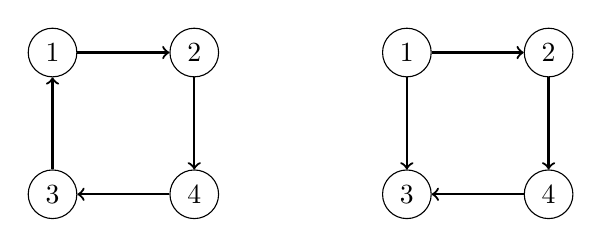
\begin{tikzpicture}[scale=0.9]
\node[draw, circle] (1) at (1,1) {$1$};
\node[draw, circle] (2) at (3,1) {$2$};
\node[draw, circle] (3) at (1,-1) {$3$};
\node[draw, circle] (4) at (3,-1) {$4$};

\path[draw,thick,->] (1) -- (2);
\path[draw,thick,->] (2) -- (4);
\path[draw,thick,->] (4) -- (3);
\path[draw,thick,->] (3) -- (1);

\node[draw, circle] (1b) at (6,1) {$1$};
\node[draw, circle] (2b) at (8,1) {$2$};
\node[draw, circle] (3b) at (6,-1) {$3$};
\node[draw, circle] (4b) at (8,-1) {$4$};

\path[draw,thick,->] (1b) -- (2b);
\path[draw,thick,->] (2b) -- (4b);
\path[draw,thick,->] (4b) -- (3b);
\path[draw,thick,->] (1b) -- (3b);
\end{tikzpicture}
\end{center}

El grafo de la derecha no es fuertemente conexo
porque, por ejemplo, no hay camino
del nodo 2 al nodo 1.

\index{strongly connected component}
\index{component graph}

Las \key{componentes fuertemente conexas}
de un grafo dividen el grafo en partes fuertemente conexas
que son lo más grandes posible.
Las componentes fuertemente conexas forman un
\key{grafo de componentes} acíclico que representa
la estructura profunda del grafo original.

Por ejemplo, para el grafo
\begin{center}
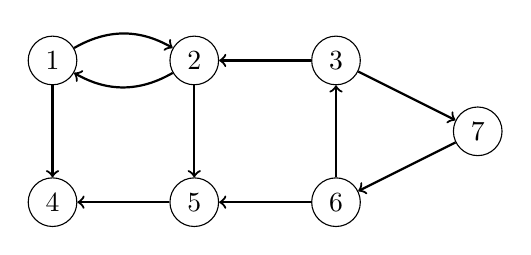
\begin{tikzpicture}[scale=0.9,label distance=-2mm]
\node[draw, circle] (1) at (-1,1) {$7$};
\node[draw, circle] (2) at (-3,2) {$3$};
\node[draw, circle] (4) at (-5,2) {$2$};
\node[draw, circle] (6) at (-7,2) {$1$};
\node[draw, circle] (3) at (-3,0) {$6$};
\node[draw, circle] (5) at (-5,0) {$5$};
\node[draw, circle] (7) at (-7,0) {$4$};

\path[draw,thick,->] (2) -- (1);
\path[draw,thick,->] (1) -- (3);
\path[draw,thick,->] (3) -- (2);
\path[draw,thick,->] (2) -- (4);
\path[draw,thick,->] (3) -- (5);
\path[draw,thick,->] (4) edge [bend left] (6);
\path[draw,thick,->] (6) edge [bend left] (4);
\path[draw,thick,->] (4) -- (5);
\path[draw,thick,->] (5) -- (7);
\path[draw,thick,->] (6) -- (7);
\end{tikzpicture}
\end{center}
las componentes fuertemente conexas son las siguientes:
\begin{center}
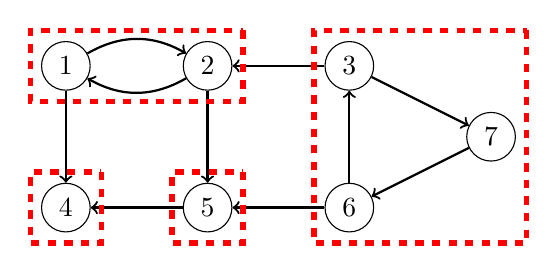
\begin{tikzpicture}[scale=0.9]
\node[draw, circle] (1) at (-1,1) {$7$};
\node[draw, circle] (2) at (-3,2) {$3$};
\node[draw, circle] (4) at (-5,2) {$2$};
\node[draw, circle] (6) at (-7,2) {$1$};
\node[draw, circle] (3) at (-3,0) {$6$};
\node[draw, circle] (5) at (-5,0) {$5$};
\node[draw, circle] (7) at (-7,0) {$4$};

\path[draw,thick,->] (2) -- (1);
\path[draw,thick,->] (1) -- (3);
\path[draw,thick,->] (3) -- (2);
\path[draw,thick,->] (2) -- (4);
\path[draw,thick,->] (3) -- (5);
\path[draw,thick,->] (4) edge [bend left] (6);
\path[draw,thick,->] (6) edge [bend left] (4);
\path[draw,thick,->] (4) -- (5);
\path[draw,thick,->] (5) -- (7);
\path[draw,thick,->] (6) -- (7);

\draw [red,thick,dashed,line width=2pt] (-0.5,2.5) rectangle (-3.5,-0.5);
\draw [red,thick,dashed,line width=2pt] (-4.5,2.5) rectangle (-7.5,1.5);
\draw [red,thick,dashed,line width=2pt] (-4.5,0.5) rectangle (-5.5,-0.5);
\draw [red,thick,dashed,line width=2pt] (-6.5,0.5) rectangle (-7.5,-0.5);
\end{tikzpicture}
\end{center}
El grafo de componentes correspondiente es el siguiente:
\begin{center}
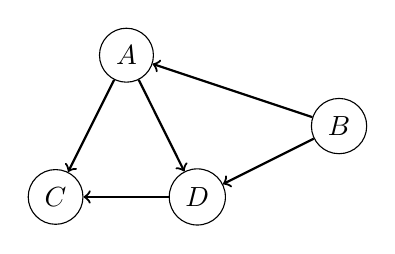
\begin{tikzpicture}[scale=0.9]
\node[draw, circle] (1) at (-3,1) {$B$};
\node[draw, circle] (2) at (-6,2) {$A$};
\node[draw, circle] (3) at (-5,0) {$D$};
\node[draw, circle] (4) at (-7,0) {$C$};

\path[draw,thick,->] (1) -- (2);
\path[draw,thick,->] (1) -- (3);
\path[draw,thick,->] (2) -- (3);
\path[draw,thick,->] (2) -- (4);
\path[draw,thick,->] (3) -- (4);
\end{tikzpicture}
\end{center}
Las componentes son $A=\{1,2\}$,
$B=\{3,6,7\}$, $C=\{4\}$ y $D=\{5\}$.

Un grafo de componentes es un grafo dirigido y acíclico,
por lo que es más fácil de procesar que el grafo original.
Como el grafo no contiene ciclos,
siempre podemos construir un orden topológico y
usar técnicas de programación dinámica como las
presentadas en el Capítulo 16.

\section{Algoritmo de Kosaraju}

\index{Kosaraju's algorithm}

El \key{algoritmo de Kosaraju}\footnote{Según \cite{aho83},
S. R. Kosaraju inventó este algoritmo en 1978
pero no lo publicó. En 1981, el mismo algoritmo fue redescubierto
y publicado por M. Sharir \cite{sha81}.} es un
método eficiente para encontrar las componentes fuertemente conexas
de un grafo dirigido.
El algoritmo realiza dos búsquedas en profundidad:
la primera búsqueda construye una lista de nodos
según la estructura del grafo,
y la segunda búsqueda forma las componentes fuertemente conexas.

\subsubsection{Búsqueda 1}

La primera fase del algoritmo de Kosaraju construye
una lista de nodos en el orden en que una
búsqueda en profundidad los procesa.
El algoritmo recorre los nodos,
y comienza una búsqueda en profundidad en cada
nodo no procesado.
Cada nodo se añadirá a la lista
después de haber sido procesado.

En el grafo de ejemplo, los nodos se procesan
en el siguiente orden:
\begin{center}
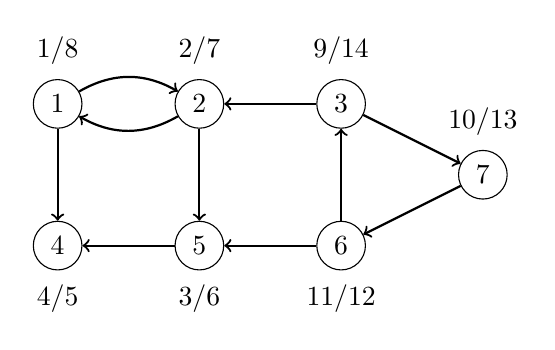
\begin{tikzpicture}[scale=0.9,label distance=-2mm]
\node[draw, circle] (1) at (-1,1) {$7$};
\node[draw, circle] (2) at (-3,2) {$3$};
\node[draw, circle] (4) at (-5,2) {$2$};
\node[draw, circle] (6) at (-7,2) {$1$};
\node[draw, circle] (3) at (-3,0) {$6$};
\node[draw, circle] (5) at (-5,0) {$5$};
\node[draw, circle] (7) at (-7,0) {$4$};

\node at (-7,2.75) {$1/8$};
\node at (-5,2.75) {$2/7$};
\node at (-3,2.75) {$9/14$};
\node at (-7,-0.75) {$4/5$};
\node at (-5,-0.75) {$3/6$};
\node at (-3,-0.75) {$11/12$};
\node at (-1,1.75) {$10/13$};

\path[draw,thick,->] (2) -- (1);
\path[draw,thick,->] (1) -- (3);
\path[draw,thick,->] (3) -- (2);
\path[draw,thick,->] (2) -- (4);
\path[draw,thick,->] (3) -- (5);
\path[draw,thick,->] (4) edge [bend left] (6);
\path[draw,thick,->] (6) edge [bend left] (4);
\path[draw,thick,->] (4) -- (5);
\path[draw,thick,->] (5) -- (7);
\path[draw,thick,->] (6) -- (7);
\end{tikzpicture}
\end{center}

La notación $x/y$ significa que
el procesamiento del nodo comenzó
en el tiempo $x$ y terminó en el tiempo $y$.
Así, la lista correspondiente es la siguiente:

\begin{tabular}{ll}
\\
nodo & tiempo de procesamiento \\
\hline
4 & 5 \\
5 & 6 \\
2 & 7 \\
1 & 8 \\
6 & 12 \\
7 & 13 \\
3 & 14 \\
\\
\end{tabular}
%
% In the second phase of the algorithm,
% the nodes will be processed
% in reverse order: $[3,7,6,1,2,5,4]$.

\subsubsection{Búsqueda 2}

La segunda fase del algoritmo
forma las componentes fuertemente conexas
del grafo.
Primero, el algoritmo invierte cada
arista del grafo.
Esto garantiza que durante la segunda búsqueda,
siempre encontraremos componentes fuertemente
conexas que no tienen nodos adicionales.

Después de invertir las aristas,
el grafo de ejemplo es el siguiente:
\begin{center}
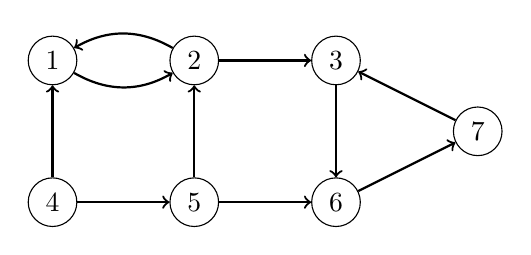
\begin{tikzpicture}[scale=0.9,label distance=-2mm]
\node[draw, circle] (1) at (-1,1) {$7$};
\node[draw, circle] (2) at (-3,2) {$3$};
\node[draw, circle] (4) at (-5,2) {$2$};
\node[draw, circle] (6) at (-7,2) {$1$};
\node[draw, circle] (3) at (-3,0) {$6$};
\node[draw, circle] (5) at (-5,0) {$5$};
\node[draw, circle] (7) at (-7,0) {$4$};

\path[draw,thick,<-] (2) -- (1);
\path[draw,thick,<-] (1) -- (3);
\path[draw,thick,<-] (3) -- (2);
\path[draw,thick,<-] (2) -- (4);
\path[draw,thick,<-] (3) -- (5);
\path[draw,thick,<-] (4) edge [bend left] (6);
\path[draw,thick,<-] (6) edge [bend left] (4);
\path[draw,thick,<-] (4) -- (5);
\path[draw,thick,<-] (5) -- (7);
\path[draw,thick,<-] (6) -- (7);
\end{tikzpicture}
\end{center}

Después de esto, el algoritmo recorre
la lista de nodos creada por la primera búsqueda,
en orden \emph{inverso}.
Si un nodo no pertenece a una componente,
el algoritmo crea una nueva componente
y comienza una búsqueda en profundidad
que añade a la nueva componente todos los nodos nuevos
encontrados durante la búsqueda.

En el grafo de ejemplo, la primera componente
comienza en el nodo 3:

\begin{center}
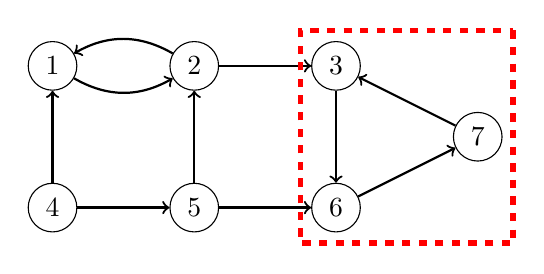
\begin{tikzpicture}[scale=0.9,label distance=-2mm]
\node[draw, circle] (1) at (-1,1) {$7$};
\node[draw, circle] (2) at (-3,2) {$3$};
\node[draw, circle] (4) at (-5,2) {$2$};
\node[draw, circle] (6) at (-7,2) {$1$};
\node[draw, circle] (3) at (-3,0) {$6$};
\node[draw, circle] (5) at (-5,0) {$5$};
\node[draw, circle] (7) at (-7,0) {$4$};

\path[draw,thick,<-] (2) -- (1);
\path[draw,thick,<-] (1) -- (3);
\path[draw,thick,<-] (3) -- (2);
\path[draw,thick,<-] (2) -- (4);
\path[draw,thick,<-] (3) -- (5);
\path[draw,thick,<-] (4) edge [bend left] (6);
\path[draw,thick,<-] (6) edge [bend left] (4);
\path[draw,thick,<-] (4) -- (5);
\path[draw,thick,<-] (5) -- (7);
\path[draw,thick,<-] (6) -- (7);

\draw [red,thick,dashed,line width=2pt] (-0.5,2.5) rectangle (-3.5,-0.5);
\end{tikzpicture}
\end{center}

Ten en cuenta que como todas las aristas están invertidas,
la componente no se ''filtra'' a otras partes del grafo.

\begin{samepage}
Los siguientes nodos de la lista son los nodos 7 y 6,
pero ya pertenecen a una componente,
por lo que la siguiente componente nueva comienza en el nodo 1:

\begin{center}
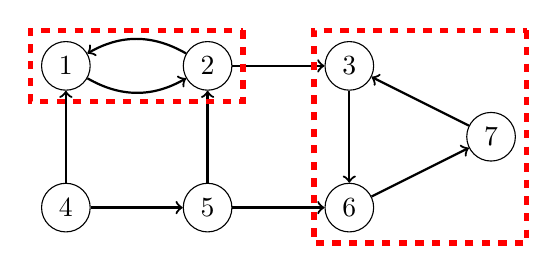
\begin{tikzpicture}[scale=0.9,label distance=-2mm]
\node[draw, circle] (1) at (-1,1) {$7$};
\node[draw, circle] (2) at (-3,2) {$3$};
\node[draw, circle] (4) at (-5,2) {$2$};
\node[draw, circle] (6) at (-7,2) {$1$};
\node[draw, circle] (3) at (-3,0) {$6$};
\node[draw, circle] (5) at (-5,0) {$5$};
\node[draw, circle] (7) at (-7,0) {$4$};

\path[draw,thick,<-] (2) -- (1);
\path[draw,thick,<-] (1) -- (3);
\path[draw,thick,<-] (3) -- (2);
\path[draw,thick,<-] (2) -- (4);
\path[draw,thick,<-] (3) -- (5);
\path[draw,thick,<-] (4) edge [bend left] (6);
\path[draw,thick,<-] (6) edge [bend left] (4);
\path[draw,thick,<-] (4) -- (5);
\path[draw,thick,<-] (5) -- (7);
\path[draw,thick,<-] (6) -- (7);

\draw [red,thick,dashed,line width=2pt] (-0.5,2.5) rectangle (-3.5,-0.5);
\draw [red,thick,dashed,line width=2pt] (-4.5,2.5) rectangle (-7.5,1.5);
%\draw [red,thick,dashed,line width=2pt] (-4.5,0.5) rectangle (-5.5,-0.5);
%\draw [red,thick,dashed,line width=2pt] (-6.5,0.5) rectangle (-7.5,-0.5);
\end{tikzpicture}
\end{center}
\end{samepage}

\begin{samepage}
Finalmente, el algoritmo procesa los nodos 5 y 4
que crean las componentes fuertemente conexas restantes:

\begin{center}
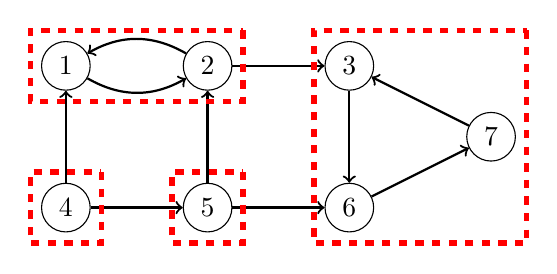
\begin{tikzpicture}[scale=0.9,label distance=-2mm]
\node[draw, circle] (1) at (-1,1) {$7$};
\node[draw, circle] (2) at (-3,2) {$3$};
\node[draw, circle] (4) at (-5,2) {$2$};
\node[draw, circle] (6) at (-7,2) {$1$};
\node[draw, circle] (3) at (-3,0) {$6$};
\node[draw, circle] (5) at (-5,0) {$5$};
\node[draw, circle] (7) at (-7,0) {$4$};

\path[draw,thick,<-] (2) -- (1);
\path[draw,thick,<-] (1) -- (3);
\path[draw,thick,<-] (3) -- (2);
\path[draw,thick,<-] (2) -- (4);
\path[draw,thick,<-] (3) -- (5);
\path[draw,thick,<-] (4) edge [bend left] (6);
\path[draw,thick,<-] (6) edge [bend left] (4);
\path[draw,thick,<-] (4) -- (5);
\path[draw,thick,<-] (5) -- (7);
\path[draw,thick,<-] (6) -- (7);

\draw [red,thick,dashed,line width=2pt] (-0.5,2.5) rectangle (-3.5,-0.5);
\draw [red,thick,dashed,line width=2pt] (-4.5,2.5) rectangle (-7.5,1.5);
\draw [red,thick,dashed,line width=2pt] (-4.5,0.5) rectangle (-5.5,-0.5);
\draw [red,thick,dashed,line width=2pt] (-6.5,0.5) rectangle (-7.5,-0.5);
\end{tikzpicture}
\end{center}
\end{samepage}

La complejidad temporal del algoritmo es $O(n+m)$,
porque el algoritmo
realiza dos búsquedas en profundidad.

\section{Problema 2SAT}

\index{2SAT problem}

La conexidad fuerte también está vinculada con el
\key{problema 2SAT}\footnote{El algoritmo presentado aquí fue
introducido en \cite{asp79}.
También existe otro algoritmo bien conocido de tiempo lineal \cite{eve75}
que se basa en vuelta atrás.}.
En este problema, se nos da una fórmula lógica
\[
(a_1 \lor b_1) \land (a_2 \lor b_2) \land \cdots \land (a_m \lor b_m),
\]
donde cada $a_i$ y $b_i$ es una variable lógica
($x_1,x_2,\ldots,x_n$)
o una negación de una variable lógica
($\lnot x_1, \lnot x_2, \ldots, \lnot x_n$).
Los símbolos ''$\land$'' y ''$\lor$'' denotan
los operadores lógicos ''y'' y ''o''.
Nuestra tarea es asignar a cada variable un valor
de modo que la fórmula sea verdadera, o indicar
que esto no es posible.

Por ejemplo, la fórmula
\[
L_1 = (x_2 \lor \lnot x_1) \land
      (\lnot x_1 \lor \lnot x_2) \land
      (x_1 \lor x_3) \land
      (\lnot x_2 \lor \lnot x_3) \land
      (x_1 \lor x_4)
\]
es verdadera cuando las variables se asignan de la siguiente manera:

\[
\begin{cases}
x_1 = \textrm{falso} \\
x_2 = \textrm{falso} \\
x_3 = \textrm{verdadero} \\
x_4 = \textrm{verdadero} \\
\end{cases}
\]

Sin embargo, la fórmula
\[
L_2 = (x_1 \lor x_2) \land
      (x_1 \lor \lnot x_2) \land
      (\lnot x_1 \lor x_3) \land
      (\lnot x_1 \lor \lnot x_3)
\]
es siempre falsa, sin importar cómo
asignemos los valores.
La razón de esto es que no podemos
elegir un valor para $x_1$
sin crear una contradicción.
Si $x_1$ es falso, tanto $x_2$ como $\lnot x_2$
deberían ser verdaderos, lo cual es imposible,
y si $x_1$ es verdadero, tanto $x_3$ como $\lnot x_3$
deberían ser verdaderos, lo cual también es imposible.

El problema 2SAT se puede representar como un grafo
cuyos nodos corresponden a
variables $x_i$ y negaciones $\lnot x_i$,
y las aristas determinan las conexiones
entre las variables.
Cada par $(a_i \lor b_i)$ genera dos aristas:
$\lnot a_i \to b_i$ y $\lnot b_i \to a_i$.
Esto significa que si $a_i$ no se cumple,
$b_i$ debe cumplirse, y viceversa.

El grafo para la fórmula $L_1$ es:
\\
\begin{center}
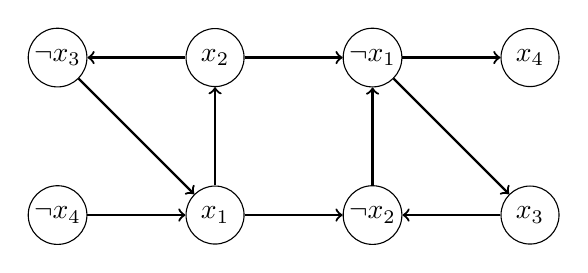
\begin{tikzpicture}[scale=1.0,minimum size=2pt]
\node[draw, circle, inner sep=1.3pt] (1) at (1,2) {$\lnot x_3$};
\node[draw, circle] (2) at (3,2) {$x_2$};
\node[draw, circle, inner sep=1.3pt] (3) at (1,0) {$\lnot x_4$};
\node[draw, circle] (4) at (3,0) {$x_1$};
\node[draw, circle, inner sep=1.3pt] (5) at (5,2) {$\lnot x_1$};
\node[draw, circle] (6) at (7,2) {$x_4$};
\node[draw, circle, inner sep=1.3pt] (7) at (5,0) {$\lnot x_2$};
\node[draw, circle] (8) at (7,0) {$x_3$};

\path[draw,thick,->] (1) -- (4);
\path[draw,thick,->] (4) -- (2);
\path[draw,thick,->] (2) -- (1);
\path[draw,thick,->] (3) -- (4);
\path[draw,thick,->] (2) -- (5);
\path[draw,thick,->] (4) -- (7);
\path[draw,thick,->] (5) -- (6);
\path[draw,thick,->] (5) -- (8);
\path[draw,thick,->] (8) -- (7);
\path[draw,thick,->] (7) -- (5);
\end{tikzpicture}
\end{center}
Y el grafo para la fórmula $L_2$ es:
\\
\begin{center}
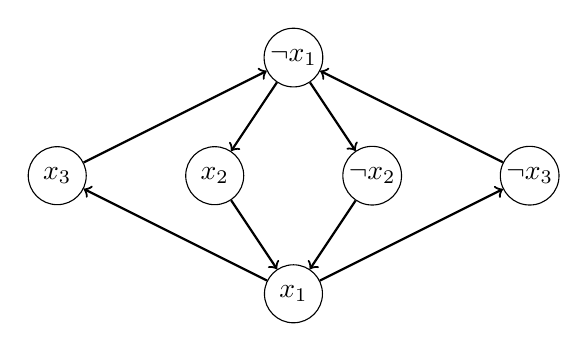
\begin{tikzpicture}[scale=1.0,minimum size=2pt]
\node[draw, circle] (1) at (1,2) {$x_3$};
\node[draw, circle] (2) at (3,2) {$x_2$};
\node[draw, circle, inner sep=1.3pt] (3) at (5,2) {$\lnot x_2$};
\node[draw, circle, inner sep=1.3pt] (4) at (7,2) {$\lnot x_3$};
\node[draw, circle, inner sep=1.3pt] (5) at (4,3.5) {$\lnot x_1$};
\node[draw, circle] (6) at (4,0.5) {$x_1$};

\path[draw,thick,->] (1) -- (5);
\path[draw,thick,->] (4) -- (5);
\path[draw,thick,->] (6) -- (1);
\path[draw,thick,->] (6) -- (4);
\path[draw,thick,->] (5) -- (2);
\path[draw,thick,->] (5) -- (3);
\path[draw,thick,->] (2) -- (6);
\path[draw,thick,->] (3) -- (6);
\end{tikzpicture}
\end{center}

La estructura del grafo nos dice si
es posible asignar los valores
de las variables de modo
que la fórmula sea verdadera.
Resulta que esto se puede hacer
exactamente cuando no hay nodos
$x_i$ y $\lnot x_i$ tales que
ambos nodos pertenezcan a la
misma componente fuertemente conexa.
Si existen tales nodos,
el grafo contiene
un camino de $x_i$ a $\lnot x_i$
y también un camino de $\lnot x_i$ a $x_i$,
por lo que tanto $x_i$ como $\lnot x_i$ deberían ser verdaderos,
lo cual no es posible.

En el grafo de la fórmula $L_1$
no hay nodos $x_i$ y $\lnot x_i$
tales que ambos nodos
pertenezcan a la misma componente fuertemente conexa,
por lo que existe una solución.
En el grafo de la fórmula $L_2$
todos los nodos pertenecen a la misma componente fuertemente conexa,
por lo que no existe una solución.

Si existe una solución, los valores de las variables
se pueden encontrar recorriendo los nodos del
grafo de componentes en orden topológico inverso.
En cada paso, procesamos una componente
que no contiene aristas que conducen a una
componente no procesada.
Si a las variables de la componente
no se les han asignado valores,
sus valores se determinarán
según los valores de la componente,
y si ya tienen valores,
permanecen sin cambios.
El proceso continúa hasta que a cada variable
se le haya asignado un valor.

El grafo de componentes para la fórmula $L_1$ es el siguiente:
\begin{center}
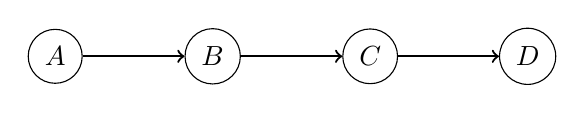
\begin{tikzpicture}[scale=1.0]
\node[draw, circle] (1) at (0,0) {$A$};
\node[draw, circle] (2) at (2,0) {$B$};
\node[draw, circle] (3) at (4,0) {$C$};
\node[draw, circle] (4) at (6,0) {$D$};

\path[draw,thick,->] (1) -- (2);
\path[draw,thick,->] (2) -- (3);
\path[draw,thick,->] (3) -- (4);
\end{tikzpicture}
\end{center}

Las componentes son
$A = \{\lnot x_4\}$,
$B = \{x_1, x_2, \lnot x_3\}$,
$C = \{\lnot x_1, \lnot x_2, x_3\}$ y
$D = \{x_4\}$.
Al construir la solución,
primero procesamos la componente $D$
donde $x_4$ se vuelve verdadero.
Después de esto, procesamos la componente $C$
donde $x_1$ y $x_2$ se vuelven falsos
y $x_3$ se vuelve verdadero.
A todas las variables se les han asignado valores,
por lo que las componentes restantes $A$ y $B$
no cambian las variables.

Ten en cuenta que este método funciona porque el
grafo tiene una estructura especial:
si hay caminos del nodo $x_i$ al nodo $x_j$
y del nodo $x_j$ al nodo $\lnot x_j$,
entonces el nodo $x_i$ nunca se vuelve verdadero.
La razón de esto es que también hay
un camino del nodo $\lnot x_j$ al nodo $\lnot x_i$,
y tanto $x_i$ como $x_j$ se vuelven falsos.

\index{3SAT problem}

Un problema más difícil es el \key{problema 3SAT},
donde cada parte de la fórmula es de la forma
$(a_i \lor b_i \lor c_i)$.
Este problema es NP-difícil, por lo que no se conoce ningún
algoritmo eficiente para resolverlo.
